\documentclass[tikz,12pt,border=12pt]{standalone}

\usepackage{mathpazo}
\usepackage[scaled=1.03,varqu]{zi4}
\usepackage[T1]{fontenc}
\usepackage[utf8]{inputenc}
\usepackage{mathtools}
\usepackage{pgf,tikz}
\usetikzlibrary{circuits.logic.US}


\begin{document}

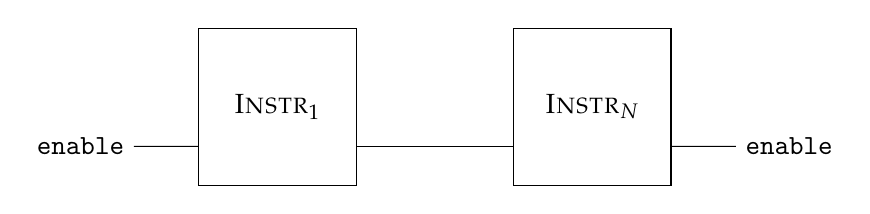
\begin{tikzpicture}[circuit logic US,%
        dot/.style    = {anchor=base,fill,circle,inner sep=1.3pt}]

\node[draw,rectangle,minimum width=2cm,minimum height=2cm] at (1,1) (i1) {$\textsc{Instr}_1$};
\node[draw,rectangle,minimum width=2cm,minimum height=2cm] at (5,1) (in) {$\textsc{Instr}_N$};
\node at (-1.5,0.5) (e_in) {\texttt{enable}};
\node at (7.5,0.5) (e_out) {\texttt{enable}};

\draw ($ (i1.east) + (0,-0.5) $) -- ($ (in.west) + (0,-0.5) $);
\draw (e_in.east) -- ($ (i1.west) + (0,-0.5) $);
\draw ($ (in.east) + (0,-0.5) $) -- (e_out.west);

\end{tikzpicture}

\end{document}



